\chapter{Integration of Microbiology with the Host Response}
\label{ch:Results3}
\textit{This chapter explores the integration of metagenomic data with host transcriptomic and genomic data in order to understand the host response in sepsis.}

\startcontents[chapters]{\vspace{-1.4cm}}
\singlespacing
\printcontents[chapters]{}{1}{\section*{ }\setcounter{tocdepth}{1}}
\doublespacing

\section{Introduction}
Application of omics-based methodologies is advancing understanding of the dysregulated host immune response to infection in sepsis. However, the frequently elusive nature of the infecting organism has limited efforts to understand the effect of disease heterogeneity involving the pathogen. This chapter explores how a better understanding of microbiology in the GAinS cohort can be applied to transcriptomic and genomic-based approaches to understand the host response in sepsis. 

\subsection{Immunosuppression in sepsis}
Over the last two decades, there has been a significant shift in our conceptual understanding of immune dysfunction in sepsis. Earlier thinking and sepsis definitions centred around the Systemic Inflammatory Response Syndrome (SIRS) and the corresponding hyperinflammatory and immune activating processes. Now, increasing evidence suggests that immunosuppression is a key disease feature, co-occuring with immune activation, and an important contributor to patient morbidity and mortality \parencite{Daviaud2015}. 

In 2001, Munford and Pugin \parencite{Munford2001} published one of the first studies demonstrating that both pro-inflammatory and anti-inflammatory processes occur rapidly after the onset of sepsis. Later, Boomer and colleagues \parencite{Boomer2011} published further evidence in the form of histological, biochemical and flow cytometric studies documenting defects in immunity in the tissues of patients dying from sepsis. T cell exhaustion, the functional impairment of effector T cells associated with decrease cytokine production, loss of proliferative capacity and decreased cytotoxicity, was described as a key mechanism in sepsis-induced immmunosuppression. 

More recently, transcriptomic studies describing sepsis endotypes have highlighted features of immunosuppression as important in distinguishing endotypes associated with worse outcome \parencite{Davenport2016} \parencite{Scicluna2017}.

\subsection{Sepsis Endotypes}
Previous work in the Knight laboratory \parencite{Davenport2016} describes two sepsis endotypes in the GAinS cohort from genome-wide gene expression analysis of peripheral blood leukocytes. Unsupervised hierarchical cluster analysis of the top 10\% most variable probes (n=2619) was performed on a discovery cohort of 265 GAinS CAP patients. Two groups were identified, Sepsis Response Signature 1 and 2 (SRS1 and SRS2). Individuals with an SRS1 endotype were characterised by features of immunosuppression, including endotoxin tolerance, T-cell exhaustion, and downregulation of HLA class II. Importantly, this group demonstrated higher 14-day mortality (discovery cohort hazard ratio 2.4, 95\% CI 1.3-4.5, p-0.005; validation cohort HR 2.8, 95\% CI 1.5-5.1, p=0.0007), supporting the observation that patients dying of sepsis show marked immunosuppression.

Similar findings were made independently by the MARS consortium \parencite{Scicluna2017}. Sepsis patients admitted to ICUs in the Netherlands were studied and four molecular endotypes (Mars1-4) were described using unsupervised consensus clustering in a discovery cohort of 306 patients from whole blood genome-wide gene expression profiling. Mars1 patients had the worst outcome, with increased 28-day mortality (HR vs all other endotypes 1.86, 95\% CI 1.21-2.86, p=0.0045). Similar to SRS1, this high-risk endotype was characterised immunosuppression, with decreased expression of genes involved in key innate and adaptive immune cell functions.

\subsection{Viral reactivation}
Studies describing a high frequency of viral reactivation in sepsis patients further support the concept that previously immunocompetent individuals can develop a varying degree of functional immunosuppression in response to severe infection. Walton and colleagues observed that 42.7\% of sepsis patients displayed viraemia with more than one reactivated virus \parencite{Walton2014}; the MARS consortium describe a 68\% frequency of herpesvirus viraemia amongst individuals with septic shock \parencite{Ong2017}. 

Reactivated viruses include the herpesviruses Epstein-Barr virus (EBV), cytomegalovirus (CMV), herpes simplex virus (HSV), and human herpesvirus 6 (HHV-6), torque teno virus (TTV), and the polyomaviruses BK and JC virus. In ICU sepsis patients, EBV is the most commonly observed reactivated virus at a frequency of 32-48\% in plasma \parencite{Walton2014} \parencite{Ong2017}. Neither study observed an association with mortality for EBV reactivation alone although the MARS consortium identified a 3.17 hazard ratio (HR) (95\% CI 1.41-7.13) for mortality with concurrent CMV and EBV reactivation \parencite{Ong2017}. In addition, Walton and colleagues observed an increased incidence of fungal infections, mean Sequential Orgain Failure Assessment (SOFA) score and ICU length of stay with EBV reactivation \parencite{Walton2014}. CMV is another commonly reactivated virus, observed at a frequency of approximately 18\% in the plasma of previously immunocompetent sepsis patients \parencite{Ong2017}. CMV reactivation has been observed to be associated with increased ICU and hospital length of stay as well as prolonged mechanical ventilation in critically ill sepsis patients \parencite{Heininger2011}.

\subsection{Epstein-Barr virus}
Like other herpesviruses, EBV is characterised by its ability to remain dormant in human cells after primary infection. Approximately 90\% of adults worldwide are EBV seropositive \parencite{Cohen2000}, the highest rate of any herpesvirus. 

Following B lymphocyte infection, latency is established with persistent infection arising due to a dynamic balance between viral evasion strategies and host immune responses. Of the 100 genes encoded by the 172Kbp EBV genome, ten are expressed during latency, establishing and maintaining the "immortalized" state. 

Whilst the viral genes and products characterising latency have been well-studied, triggers for the shift from latency to lytic replication and reactivation are not clearly defined. In general, reactivation disease is not believed to be a marked issue with EBV (unlike other herpesviruses, e.g. CMV) apart from in the context of post-transplant lymphoproliferative disorders.

\subsection{Transcriptomic signatures of viral infection}
\label{sssec:emmaDEgenes}
\textbf{GAinS dataset.} Previous work done in the Knight laboratory by Dr Emma Davenport included the definition of gene expression signatures for different infection types in the GAinS CAP cohort /parencite{Davenport2014}. Four contrasts were made with differentially expressed probes defined as those with a FDR $<$0.05 and a modest fold change $>$1.2. The contrasts made are summarised in Table \ref{tab:emmaDEgenes}. 

\FloatBarrier
\begin{table}[]
\begin{center}
\begin{tabular}{|c|c|l|}
\hline
\textbf{Comparison (no. of patients)} & \textbf{Patients} & \textbf{Differentially expressed probes} \\ \hline
Viral (25) vs no viral (239)          & 264               & 66                                       \\ \hline
H1N1 (16) vs other viral (9)          & 25                & 0                                        \\ \hline
Viral (23) vs bacterial (75)          & 98                & 2                                        \\ \hline
Gram+ (47) vs Gram- (25)              & 72                & 0                                        \\ \hline
\end{tabular}

\end{center}
\smallskip
\caption[Previous work transcriptomic signatures for microbiology] {\textbf{Previous work: differential gene expression analysis for various classes of infection.} Genome-wide gene expression data from microarray was analysed in patients with sepsis due to CAP. Differential expression analysis was performed for different microbiological classes of infection. Differentially expressed probes are defined as those with FDR $<$0.05 and fold change $>$1.2.} 
\label{tab:emmaDEgenes}
\end{table}


Of interest is the viral vs no viral infection  analysis, which identified 66 differentially expressed probes. These mapped to 54 genes in Ingenuity Pathway Analysis (IPA) with enrichment of pathways involving the role of pattern recognition receptors (PRRs) in recognition of viruses and the activation of interferon-regulatory factors (IRF) by cytosolic PRRs.

A prediction model for viral infection was defined using the GeneRave R package (CSIRO Bioinformatics R package version 3.0.8) \parencite{Kiiveri2008}. To reduce the number of possible predictors, only probes that were differentially expressed at FDR $<$0.05 and fold change $>$1.2, mapped to genes in IPA and were moderate to highly expressed (expression $>$6.5) in a proportion of samples equating to the smallest group of the comparison were used. Six genes were selected for the prediction model: \textit{IFI27, TGIF2, LY6E, CCNY, DYNLL2,} and \textit{LAMP3}. Using leave-one-out cross-validation, a ROC curve (AUC 0.89) and MR (9.1) was determined for the model.

Limitations of this analysis include the lack of accurate microbiological phenotyping in the comparator "non-viral" group. The electronic case record forms (eCRF) only provides information where testing yields a positive result, thus we are unable to confirm cases where testing has yielded a negative result. As viral testing is typically only performed during influenza outbreaks, there is a high likelihood the "non-viral" group included cases of undiagnosed viral infection. This may explain why only 66 differentially expressed probes were identified at a modest fold change of 1.2. 

\textbf{Other datasets.} A number of published studies have described gene signatures differentiating viral from bacterial infection. Two examples include the seven-gene set described by Sweeney \textit{et al} \parencite{Sweeney2016} and the two-gene disease risk score (DRS) described by Herberg \textit{et al} \parencite{Herberg2016}.

Sweeney and colleagues \parencite{Sweeney2016} combined 8 datasets from adults and children with CAP, febrile illness and/or sepsis to form a discovery dataset of 426 individuals (n=142 viral; n=284 bacterial). Gene expression was analysed from whole blood or peripheral blood mononuclear cells. The authors performed differential expression analysis and identified 72 genes with a FC >2 and FDR <0.01. A greedy forward search method was then utilised to identify a set of seven genes which discriminated viral from bacterial infection. This included three "viral" genes (/textit{IFI27, JUP, LAX1}) and four "bacterial" genes (\textit{HK3, TNIP1, GPAA1, CTSB}). ROC analysis was performed with an AUC value of 97\% (95\% CI: 89\%-99\%) in the discovery cohort. The gene set was subsequently validated in a combined validation cohort consisting six datasets of 341 individuals (n=203 viral; n=138 bacterial). Here, it performed with an AUC value of 91\% (95\% CI 82\%-96\%). 

Herberg and colleagues \parencite{Herberg2016} prospectively recruited febrile children presenting to hospital. Genome-wide gene expression analysis was performed on RNA extracted from whole blood. Differential gene expression analysis identified 285 probes differentially expressed at a FC >2 and FDR <0.05. The elastic net method \parencite{Zou2005} was used to identify 38 probes from initial gene set. Elastic net is a variable selection algorithm that is an alternative to standard linear regression with least squares fitting, particularly suited to cases where the number of predictors greatly exceeds the number of observations. Elastic net combines the lasso and ridge regression methods of shrinkage, minimising the number of variables included (lasso) whilst also making the model less dependent on any one variable (ridge).

Subsequently, forward selection-partial least squares was used to eliminate highly correlated transcripts and a two transcript signature was identified. This involved a ratio of \textit{IFI44L} expression to \textit{FAM89A} expression, which the authors termed a disease risk score (DRS). ROC analysis was performed, yielding an AUC of 96.3\% (95\% CI 87.4\%-100\%) in the test dataset of 29 individuals and an AUC of 97.4\% (95\% CI 91.2\%-100\%) in the validation dataset of 51 individuals. 

\subsection{HLA}
The extreme variability seen in the Major Histocompatibility Complex (MHC) region is believed to have arisen due to human-viral co-evolution. It is unsurprising therefore, that associations are seen between specific HLA alleles and infectious disease susceptibility, progression and outcome. 

Notable examples include human immunodeficiency virus 1 (HIV-1), hepatitis B virus (HBV) and hepatitis C virus (HCV) infection. In HIV-1 infection, Carrington and colleagues \parencite{Carrington1999} tested 63 alleles and found six (A*29, B*27, B*35, B*41, Cw*04 and Cw*12) to be significantly associated with disease progression in Caucasians. In addition, elevated \textit{HLA-A} expression levels were found to be negatively correlated with control of HIV infection \parencite{Ramsuran2018}. In HBV infection, Nishida and colleagues \parencite{Nishida2016} tested 144 alleles and found DQB1*06:01 to have the strongest association with susceptibility to chronic infection in Japanese individuals. Finally, in HCV infection, B*27 \parencite{Neumann-Haefelin2006} and B*57 \parencite{Kim2011} have both been found to be associated with a higher rate of viral clearance. 

In addition, genome-wide association studies (GWAS) and genome-wide linkage studies (GWLS) have identified polymorphisms in the HLA regions to be associated with viral (HIV, HBV, HCV), bacterial (leprosy, tuberculosis), and parasitic (malaria, leishmaniasis, and schistosomiasis) infections \parencite{Blackwell2009}. For example, the International HIV Controllers Study \parencite{Pereyra2010} identified over 300 genome-wide significant SNPs within the MHC to be associated with control of HIV-1 whilst the first GWAS of leprosy susceptibility reported associations with SNPs in six genetic loci, including the HLA-DR region \parencite{Zhang2009}.  

In summary, these examples in the literature suggest it would be of particular interest to investigate the association between specific HLA alleles and susceptibility to different microbiological classes of sepsis. 

\subsection{Aims}
The overall aim of this chapter is to explore how improved resolution of microbiology in the sepsis cohort can be applied to transcriptomic and genomic-based approaches to understand the host response in sepsis. Specifically, the most commonly identified bacterial (\textit{Streptococcus pneumoniae}) and viral (influenza) infections will be studied as well as the most commonly reactivated virus (Epstein Barr virus). These will be related to Sepsis Response Signature endotype, total leukocyte gene expression and underlying host genotype (HLA type). Specific aims are as follows.

\begin{enumerate}
	\item To characterise the extent and implications of EBV reactivation and integrate this with host transcriptomic data.
	\item To investigate the association between \textit{Streptococcus pneumoniae} bacterial load and sepsis endotype (SRS status).
	\item To describe host transcriptomic signatures of viral infection, influenza infection, and \textit{Streptococcus pneumoniae} infection and identify predictive gene sets for these infections.
	\item To investigate the association between host genotype (HLA type) and susceptibility to different classes of infection.
\end{enumerate}

\section{Results}
\subsection{QC, normalisation and combination of microarray datasets}
In this chapter, I analyse microarray gene expression data from the GAinS study processed in four batches over a six year period. These include samples from patients with sepsis due to CAP or faecal peritonitis (FP) enrolled through the GAinS study, recruited from 34 participating ICUs between 2005 and 2016. Serial samples were obtained on the first, and/or third, and/or fifth day of ICU admission. The total peripheral blood leukocyte population was isolated from whole blood for RNA extraction using the LeukoLOCK system (Invitrogen).

All four of these datasets were generated by former DPhil students in the Knight lab: Radhakrishnan 2010, Dr Jayachandran Radhakrishnan; Davenport 2011, Dr Emma Davenport; Burnham 2014, Dr Katie Burnham; Burnham 2016, Dr Katie Burnham. Samples from cardiac surgery patients (sepsis control patients) were taken prior to and after their operation, and included in the two earlier cohorts. These samples were processed by Dr Eduardo Svoren (Barts and the London).

Genome-wide gene expression data was generated for all four cohorts using the Illumina Human-HT-12 v4 Expression BeadChip (47,231 probes). The data QC and normalisation was performed for each dataset in parallel. This was performed by myself for the Radhakrishnan 2010 and Davenport 2011 datasets, and by Dr Katie Burnham for the Burnham 2014 and Burnham 2016 datasets. Table \ref{tab:gex-summary} summarises the samples included in each dataset following QC. Following QC of each dataset, the four datasets were combined.

\begin{table}[]
\begin{center}
\begin{tabular}{|l|l|l|l|l|}
\hline
\textbf{Dataset}   & \textbf{\begin{tabular}[c]{@{}l@{}}Samples \\ post-QC\end{tabular}} & \textbf{CAP}    & \textbf{FP}   & \textbf{Cardiac} \\ \hline
Radhakrishnan 2010 & 236                                                                 & 124 (39/45/40)  & 94 (37/34/23) & 18 (6/6/6)       \\ \hline
Davenport 2011     & 339                                                                 & 262 (130/86/46) & 0             & 77 (39/0/38)     \\ \hline
Burnham 2014       & 159                                                                 & 106 (42/42/22)  & 53 (25/15/13) & 0                \\ \hline
Burnham 2016       & 143                                                                 & 72 (24/24/24)   & 71 (23/24/24) & 0                \\ \hline
\textbf{Total}     & \textbf{877}                                                        & \textbf{564}    & \textbf{218}  & \textbf{95}      \\ \hline
\end{tabular}
\end{center}
\smallskip
\caption[Summary of microarray datasets]{\textbf{Summary of microarray datasets}. Numbers in brackets refer to samples at each timepoint. The three timepoints for the sepsis patients are day 1, day 3 and day 5 after ICU admission. The three timepoints for the cardiac surgery patients are pre-operative, immediately post-operative, 24 hours post-operative.}
\label{tab:gex-summary}
\end{table}

\textbf{Radhakrishnan 2010}
The Radhakrishnan 2010 dataset (n=264) \parencite{Radhakrishnan2012} included 234 samples from 138 sepsis patients and 30 samples from 10 cardiac surgery patients. Twenty-two samples were excluded prior to data normalisation (3 samples from a patient subsequently discovered as failing to meet study inclusion criteria; 2 mislabelled samples; 5 technical replicates; 12 samples from cardiac surgery patients with missing consent forms). 

Six outlying samples were identified through Principal Component Analysis (PCA and other QC measures (Figure \ref{fig:PCAJay}) and excluded. Probes that did not have a detection p-value $<$0.05 in at least 5\% of samples were removed (19,978 probes). Following normalisation and QC, expression data was available for 27,253 probes in 236 samples (124 CAP, 94 FP, 18 cardiac surgery) from 143 patients (73 CAP, 64 FP, 6 cardiac surgery).

\FloatBarrier
\begin{figure}[htbp]
\centering
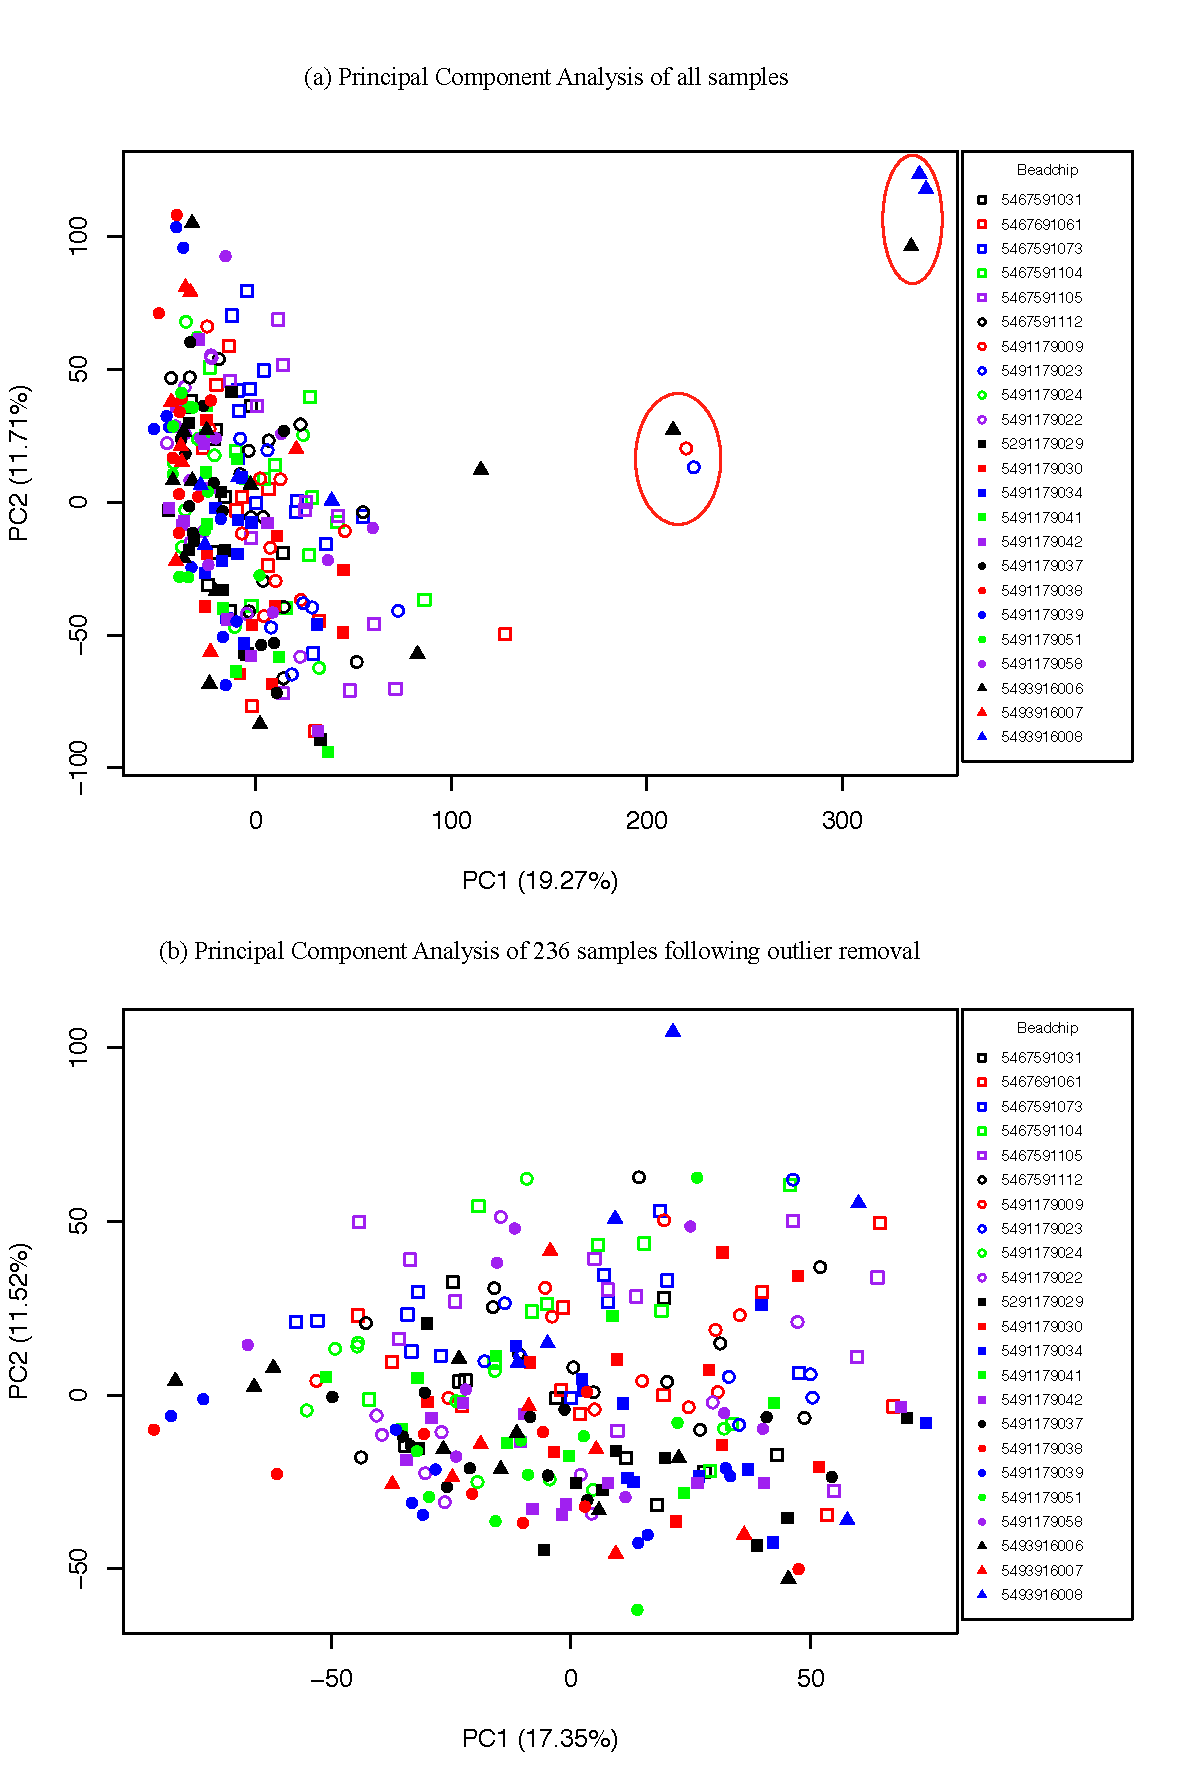
\includegraphics[scale=0.7]{./Results3/Images/PCA_Radhakrishnan2010.pdf}
\caption[Principal Component Analysis: Radhakrishnan 2010]{\textbf{Principal Component Analysis: Radhakrishnan 2010} The first two principal components of the gene expression data are plotted, with the amount of variance explained by each noted; (a) when all samples are included in the analysis, and (b) after the removal of six outliers. Samples are coloured according to beadchip and outlying samples are circled in red.}
\label{fig:PCAJay}
\end{figure}

\textbf{Davenport 2011}
The Davenport 2011 dataset has been published as the discovery cohort in \cite{Davenport2016}. This initial dataset (n=432) included 306 samples from 306 CAP patients and 126 samples from 63 cardiac surgery patients. Eighty-five samples were excluded prior to data normalisation (48 samples from 4 chips with failed hybridisation; 34 samples from cardiac surgery patients with missing consent forms; 1 patient subsequently discovered as failing to meet study inclusion criteria; 1 patient who withdrew consent; 1 patient with suspected active leukaemia). 

Eight outlying samples were identified through PCA and other QC measures (Figure \ref{fig:PCAEmma}) and excluded. Probes that did not have a detection p-value $<$0.05 in at least 5\% of samples were removed (20,805 probes). Following normalisation and QC, expression data was available for 26,426 probes in 339 samples (262 CAP, 77 cardiac surgery) from 301 patients (262 CAP, 39 cardiac surgery).

\FloatBarrier
\begin{figure}[htbp]
\centering
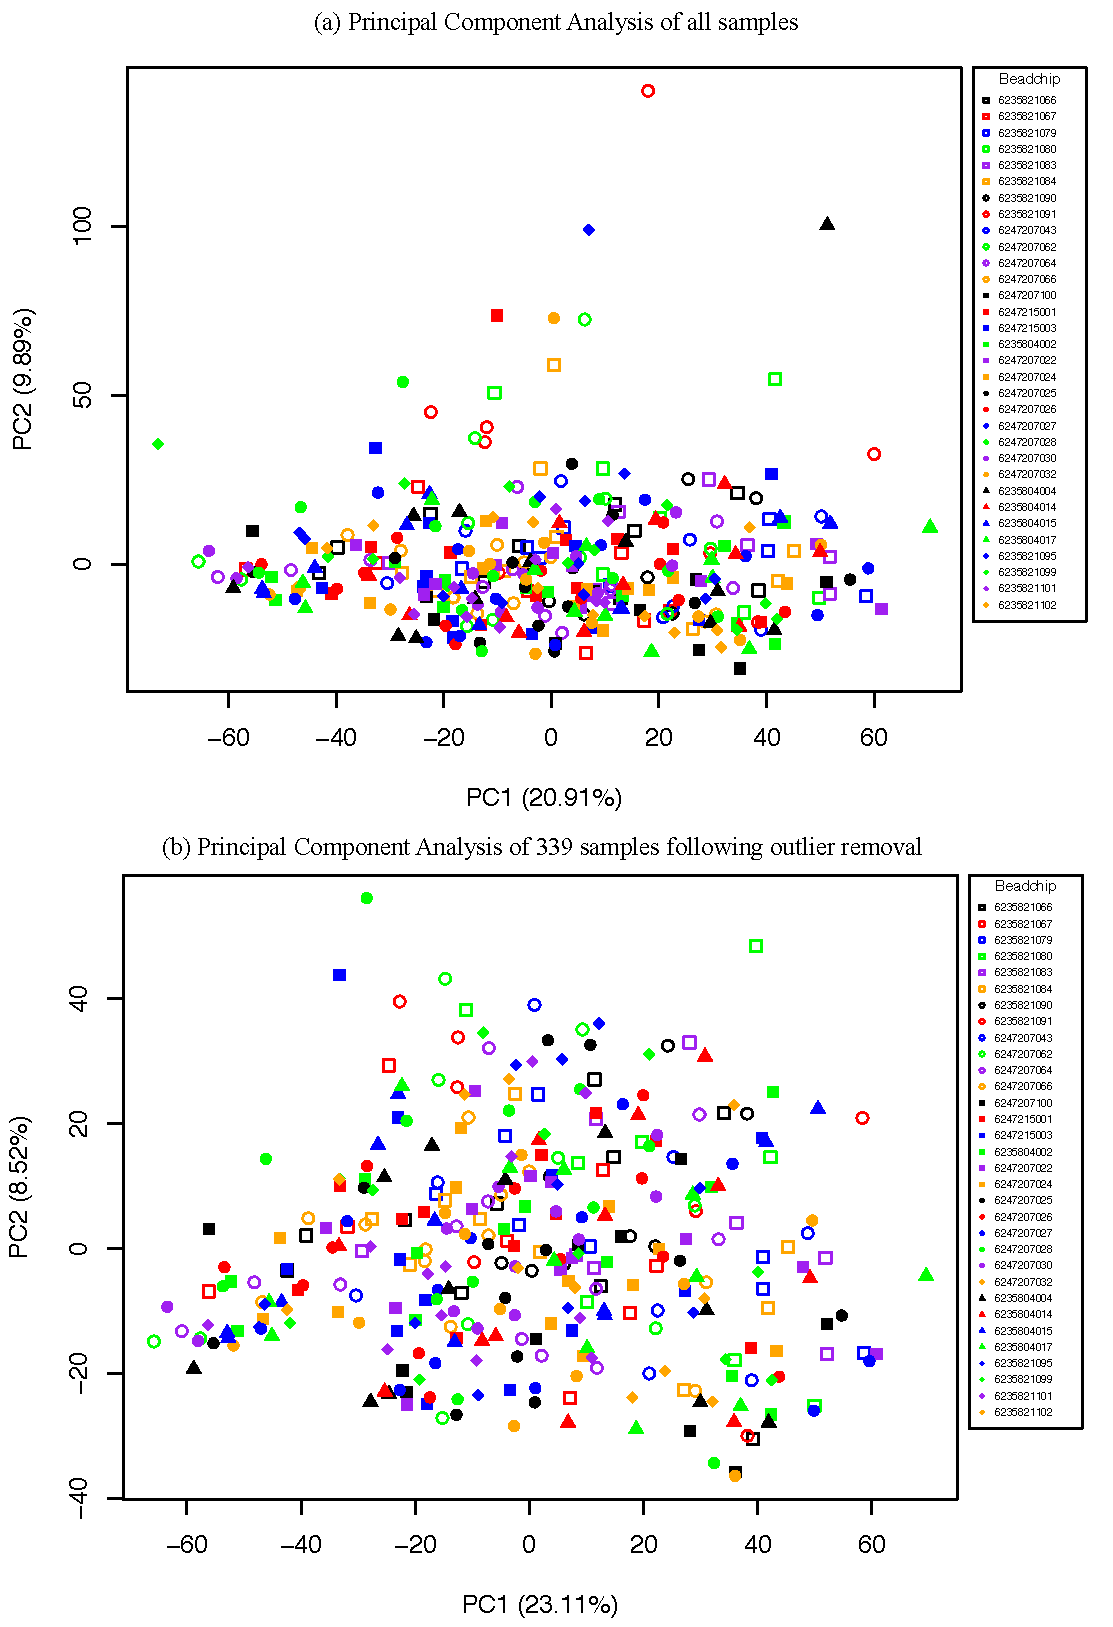
\includegraphics[scale=0.75]{./Results3/Images/PCA_Davenport2011.pdf}
\caption[Principal Component Analysis: Davenport 2011]{\textbf{Principal Component Analysis: Davenport 2011} The first two principal components of the gene expression data are plotted, with the amount of variance explained by each noted; (a) when all samples are included in the analysis, and (b) after the removal of eight outliers. Samples are coloured according to beadchip and outlying samples are circled in red.}
\label{fig:PCAEmma}
\end{figure}

\textbf{Burnham 2014}
Data QC and normalisation was carried out by Dr Katie Burnham \parencite{Burnham2017}. Post-QC, this dataset was comprised of 159 samples (106 CAP, 53 FP) from the same number of patients.

\textbf{Burnham 2016}
Data QC and normalisation was carried out by Dr Katie Burnham \parencite{Burnham2017}. Post-QC, this dataset was comprised of 143 samples (72 CAP, 71 FP) from 48 patients (24 CAP, 24 FP).

\textbf{Combination of datasets}
Following separate QC and normalisation, the four datasets were combined. There were 92 additional probes in the two more recent datasets, which were removed. In addition, there were 61 samples that were repeated in the Davenport 2011 dataset following initial analysis in the Radhakrishnan dataset. Given that the SRS endotypes were defined and published for the Davenport 2011 dataset, the samples in this dataset were retained and duplicates in the Radhakrishnan 2010 dataset removed. Probes that did not have a detection p-value $<$0.05 in at least 5\% of samples were removed (19,003 probes). Data was then normalised before the ComBat function from the R package sva applied to remove known batch effects (Figure \ref{fig:combat}). In this combined dataset, expression data was available for 28,228 probes for 816 samples (509 CAP, 218 FP, 89 cardiac surgery) from 591 patients (408 CAP, 141 FP, 42 cardiac surgery).

\FloatBarrier
\begin{figure}[htbp]
\centering
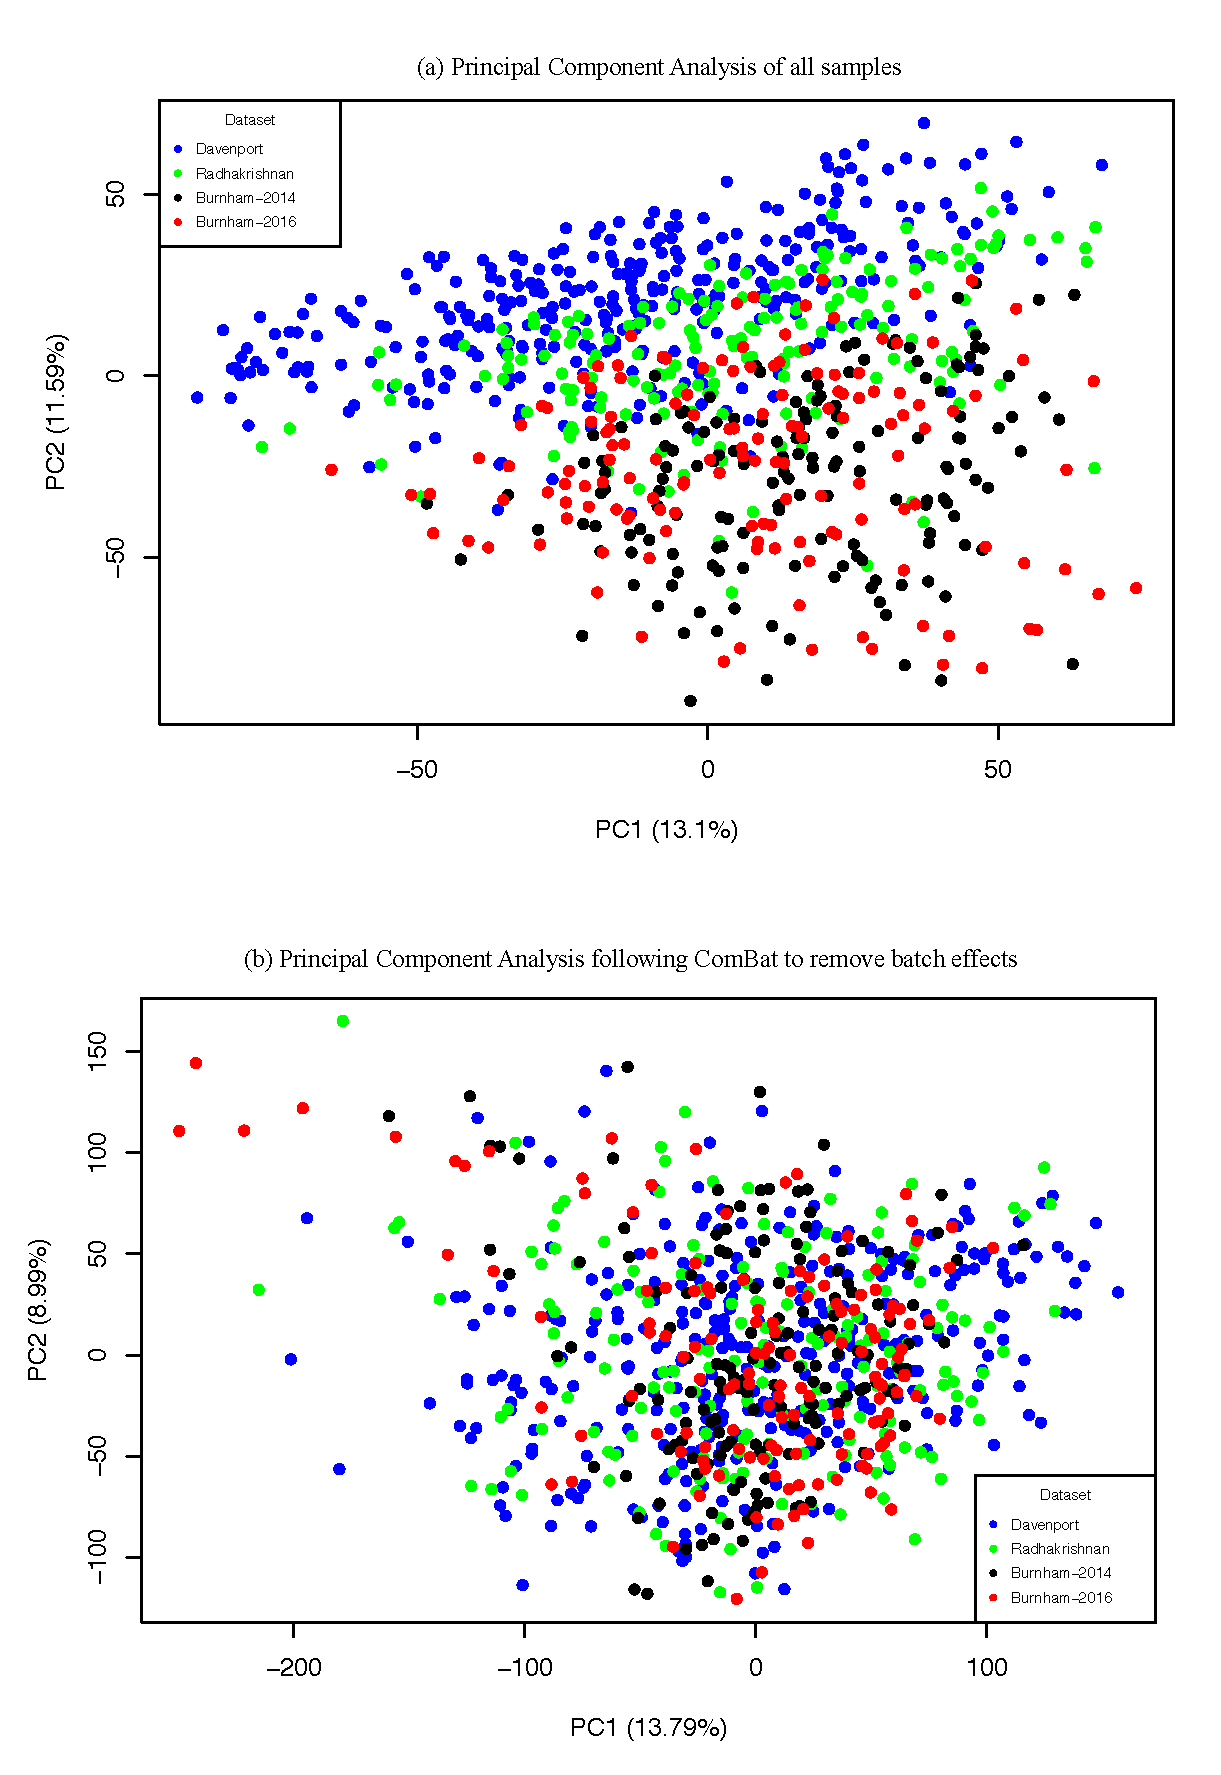
\includegraphics[scale=0.7]{./Results3/Images/PCA_alldata.pdf}
\caption[Principal Component Analysis: Combined dataset]{\textbf{Principal Component Analysis: Combined dataset of 816 samples from GAinS CAP and FP patients.} The first two principal components of the gene expression data are plotted, with the amount of variance explained by each noted; (a) prior to batch effects being removed (b) after removal of batch effects by ComBat. Samples are coloured according to the four datasets: Radhakrishnan (n=175), Davenport (n=339), Burnham-2014 (n=159), Burnham-2016 (n=143).}
\label{fig:combat}
\end{figure}

\subsection{Evidence for immunosuppression: viral reactivation}
Immunosuppression is a key pathophysiological process in sepsis, with viral reactivation seen as a consequence. Amongst 757 samples from 573 GAinS patients with CAP undergoing metagenomic sequencing (defined here as the metagenomic cohort), viral reactivation was observed in 24\% of individuals, with EBV the most commonly observed virus (Table ~\ref{tab:viralreactivation}). Notably, this was observed despite there being an enrichment for earlier time points from ICU admission (Day 1=302; Day 3=284; Day 5=171). Six individuals showed simultaneous reactivation of EBV and a second virus. 

\begin{table}[]
\begin{center}
\begin{tabular}{|c|c|c|c|c|c|}
\hline
\begin{tabular}[c]{@{}c@{}}Other reactivated\\ virus\end{tabular} & None       & HSV       & CMV       & HHV-6     & JC virus  \\ \hline
\begin{tabular}[c]{@{}c@{}}EBV-negative \\ (n=438)\end{tabular}   & 422 (74\%) & 5 (0.9\%)                                                      & 1 (0.2\%)       & 8 (1.4\%)                                                      & 2 (0.3\%) \\ \hline
\begin{tabular}[c]{@{}c@{}}EBV-positive\\ (n=135)\end{tabular}    & 129 (23\%) & 4 (0.7\%)                                                      & 1 (0.2\%)       & 0 (0\%)                                                        & 1 (0.2\%) \\ \hline
\end{tabular}
\end{center}
\smallskip
\caption[Incidence of viral reactivation]{\textbf{Incidence of viral reactivation in the metagenomic cohort (n=573)}. Six patients demonstrated reactivation with EBV and a second virus.}
\label{tab:viralreactivation}
\end{table}
\FloatBarrier

As the incidence of CMV reactivation was unexpectedly low, droplet digital PCR was carried out on a subset of samples overlapping with the metagenomic cohort (n=98). Samples were selected based on: (a) host transcriptomic data availability (overlap with Davenport 2011 cohort); (b) CMV positivity from metagenomics (n=1); and (c) sample availability. Of the 98 samples assayed, only two were positive for CMV including the one positive sample identified by metagenomics. The second sample (missed by metagenomics) was positive for CMV at a low level (86 copies/ml).

\subsection{Evidence for immunosuppression: EBV}
\label{sssec:ebv}
\textbf{Cohort description.}
EBV was assayed from plasma samples taken at one or more time points (day 1 and/or day 3 and/or day 5 of ICU admission) by two methods, targeted metagenomics (757 samples from 573 patients) and digital droplet PCR (ddPCR) (619 samples from 565 patients), forming the two cohorts for this section. Targeted metagenomics enabled characterisation of multiple reactivated viruses in plasma, whilst ddPCR enabled a quantitative approach focused on EBV, enabling assessment of individuals from the metagenomic cohort at later time points as well as additional individuals. There was an overlap of 409 patients in the application of the two methods, with a total of 731 patients evaluated overall.

\textbf{Serology.}
Plasma from 40 EBV ddPCR-positive patients, selected to represent the full range of viral loads observed, were tested for IgG and IgM antibodies against EBV Viral Capsid Antigen (VCA). All individuals tested (n=40; 100\%) were positive for the IgG VCA antibody and negative for IgM VCA antibody, indicating that sepsis had coincided with viral reactivation and not primary infection.

\textbf{Incidence of reactivation with time after ICU admission.}
Combining both cohorts, a total of 1042 unique samples (731 patients) from days 1,3 and 5 after ICU admission were evaluated by either targeted metagenomics, ddPCR, or both. Where the ddPCR and metagenomic result differed (15\% of samples), the positive result was taken forward for further analysis. The overall incidence of EBV reactivation at any time point was 37\% (271/731). The incidence of EBV reactivation increased significantly over time ($\chi^2$=24.6; d.f.=2; p=4.6 x 10$^{-6}$) (Table ~\ref{tab:ebvincidence}).

\FloatBarrier
\begin{table}[]
\begin{center}
\begin{tabular}{|c|c|c|c|}
\hline
\textbf{Day of sampling} & \textbf{EBV negative} & \textbf{EBV positive} & \textbf{Total} \\ \hline
1                        & 245 (75\%)            & 82 (25\%)             & 327            \\ \hline
3                        & 247 (70\%)            & 106 (30\%)            & 353            \\ \hline
5                        & 209 (58\%)            & 153 (42\%)            & 362            \\ \hline
\end{tabular}
\end{center}
\smallskip
\caption[EBV status by day of sampling]{\textbf{EBV status by day of sampling after ICU admission.} GAinS patients with sepsis due to CAP had their EBV status evaluated by targeted metagenomic analysis or ddPCR of plasma samples obtained on days 1, 3 and/or 5 of ICU admission.}
\label{tab:ebvincidence}
\end{table}

\textbf{Clinical outcomes.}
Clinical outcome data was compared between EBV-negative (n=460) and EBV-positive (n=271) individuals (Table ~\ref{tab:ebvoutcome}); patients were considered EBV-positive if at least one sample at any time point was positive by ddPCR or targeted metagenomics. Twenty-eight-day mortality was higher (27\% vs 20\%; p=0.04) and ICU length of stay was longer (12.9 days vs 9.2 days; p=0.004) in the EBV-positive group. In addition, the EBV-positive group had more organ failures with higher day 1 Sequential Organ Failure Assessment (SOFA) scores (6.9 vs 5.9; p=0.00011) and maximum SOFA scores (7.9 vs 6.7; p=3.6 x 10$^{-6}$).

\begin{table}[]
\begin{center}
\begin{tabular}{|c|c|c|c|}
\hline
\textbf{Characteristic}     & \textbf{\begin{tabular}[c]{@{}c@{}}EBV-negative\\ (n=460)\end{tabular}} & \textbf{\begin{tabular}[c]{@{}c@{}}EBV-positive\\ (n=271)\end{tabular}} & \textbf{p-value} \\ \hline
Age                         & 60.5 (17-92)                                                            & 62.4 (19-91)                                                            & 0.11             \\ \hline
Male sex\textasciicircum{}  & 275 (60\%)                                                              & 141 (52\%)                                                               & 0.049             \\ \hline
Mortality (28-day)`         & 92 (20\%)                                                               & 72 (27\%)                                                               & 0.040             \\ \hline
ICU length of stay`         & 9.2 & 12.9 & 0.0040            \\ \hline
SOFA score (day 1)*         & 5.9 & 6.9 & 0.00011           \\ \hline
SOFA score (maximum)*       & 6.7 & 7.9                                                                     & 3.6 x 10$^{-6}$           \\ \hline
\end{tabular}
\end{center}
\smallskip
\caption[EBV and clinical outcomes]{\textbf{Clinical characteristics and outcome data compared between EBV-negative and EBV-positive GAinS patients with sepsis due to CAP (total n=731).} ICU length of stay analysis only includes patients surviving to ICU discharge. T-test performed except where indicated (\textasciicircum{}Chi-squared test; *Mann-Whitney U-test; `Log-rank test).} 
\label{tab:ebvoutcome}
\end{table}
\FloatBarrier

\textbf{Association with SRS endotype.} 
SRS group membership (determined at the first available time point after ICU admission) was evaluated in the context of EBV positivity over the first 5 days of ICU admission. Considering SRS endotype as a categorical trait, there was a greater proportion of SRS1 patients within the EBV-positive group (44\% vs 35\%; p=0.097) but this was not statistically significant (Table ~\ref{tab:ebv-gex}). However, this binary classification is a simplification of what is a continuous spectrum of gene expression patterns, with some individuals at either extreme and others with more moderate SRS signatures in the centre. Therefore, we reasoned that considering SRS endotype as a continuous trait might increase statistical power to detect an association with EBV-positivity.

\begin{table}[]
\begin{center}
\begin{tabular}{|c|c|c|c|}
\hline
\textbf{Characteristic}                       & \textbf{\begin{tabular}[c]{@{}c@{}}EBV-negative \\ (n=239)\end{tabular}} & \textbf{\begin{tabular}[c]{@{}c@{}}EBV-positive \\ (n=152)\end{tabular}} & \textbf{p-value} \\ \hline
Age                                           & 63.5 (19-91)                                                             & 63.5 (17-91)                                                             & 1.00             \\ \hline
Male sex\textasciicircum{}                    & 149 (62\%)                                                               & 88 (58\%)                                                                & 0.44             \\ \hline
Sepsis Response Signature 1\textasciicircum{} & 84 (35\%)                                                                & 67 (44\%)                                                                & 0.097            \\ \hline
Mortality (28-day)'                           & 69 (29\%)                                                                & 53 (35\%)                                                                & 0.20             \\ \hline
ICU length of stay'                           & 10.7                                                                     & 13.4                                                                     & 0.070            \\ \hline
SOFA score (day 1)*                           & 6.2                                                                      & 7.0                                                                      & 0.019            \\ \hline
SOFA score (maximum)*                         & 7.1                                                                      & 8.1                                                                      & 0.0066           \\ \hline
\end{tabular}
\end{center}
\smallskip
\caption[EBV and clinical outcomes]{\textbf{Clinical characteristics and outcome data compared between EBV-negative and EBV-positive GAinS patients with sepsis due to CAP with gene expression data available.}ICU length of stay analysis only includes patients surviving to ICU discharge. T-test performed except where indicated (\textasciicircum{}Chi-squared test; *Mann-Whitney U-test; `Log-rank test).} 
\label{tab:ebv-gex}
\end{table}
\FloatBarrier

The difference in gene expression between SRS1 and SRS2 individuals can be observed in the first principal component (PC1) of principal component analysis (PCA) of the top 10\% most variable genes (Figure ~\ref{fig:pc1}). Thus, we compared PC1 between EBV-positive and EBV-negative individuals and found EBV-positive individuals had lower PC1 values, i.e. a more SRS1-like gene expression (Figure ~\ref{fig:ebvsrs}) (mean PC1 score -2.8 vs 1.8; p=0.014; t-test).

\FloatBarrier
\begin{figure}[htbp]
\centering
\includegraphics[scale=0.6]{./Results3/Images/PC1.pdf}
\caption[Principal Component 1]{\textbf{Principal Component 1} Principal component analysis was performed on the top 10\% most variable genes expressed by peripheral blood leukocytes in GAinS patients with sepsis due to CAP. Individuals with both gene expression data and known EBV status (n=391) are included here with the first principal component (PC1) plotted against SRS endotype.}
\label{fig:pc1}
\end{figure}


\begin{figure}[htbp]
\centering
\includegraphics[scale=0.6]{./Results3/Images/SRS_jitter.pdf}
\caption[EBV-positivity and SRS status]{\textbf{Boxplot of first available SRS as a continuous trait against EBV status over the first five days of ICU admission.} GAinS patients with sepsis due to CAP for whom gene expression data and EBV status are avaiable are included here (n=391). The values for principal component 1 (PC1) provide a continuous measure of SRS endotype with higher values representing an SRS2 endotype and lower values representing an SRS1 endotype. }
\label{fig:ebvsrs}
\end{figure}
\FloatBarrier

\textbf{Levels of EBV viraemia.} 
Digital droplet PCR was used to assay EBV in plasma samples (619 samples; 565 patients) over the first five days of admission (days 1,3, and/or 5). The maximum EBV load was related to SRS endotype determined from the first available timepoint after ICU admission (Figure ~\ref{fig:ebvload}). The median EBV load was higher in the SRS1 compared to the SRS2 endotype patients (211 vs 106 copies/ml; p=0.025; Mann-Whitney U-Test). Thus, among those in whom the virus was detected, the two SRS endotypes differed in the amount of EBV measured.

\FloatBarrier
\begin{figure}[htbp]
\centering
\includegraphics[width=\textwidth]{./Results3/Images/ebvload.pdf}
\caption[EBV load and SRS status]{\textbf{Boxplot of maximum EBV load over the first 5 days of ICU admission (ddPCR) against first available SRS status after ICU admission.} GAinS patients with sepsis due to CAP were analysed with respect to EBV viral load by ddPCR and SRS endotype by genome-wide gene expression microarray analysis from peripheral blood leukocytes.}
\label{fig:ebvload}


\end{figure}
\FloatBarrier

\textbf{Gene expression signature.} 
Global gene expression from the peripheral blood total leukocyte population was compared between EBV-positive and EBV-negative individuals (Figure ~\ref{fig:ebvsig1}). The differential expression analysis included only gene expression from patient samples at the first available time point; 28228 probes were tested. Nine genes were differentially expressed at a fold-change $>$1.5 and FDR $<$0.05 (Table ~\ref{tab:ebv-de-genes}). These include \textit{CACNA2D3} (FDR 0.00521, fold change 1.55, downregulated in EBV-positive patients) which is a tumour suppressor gene downregulated in primary nasopharyngeal cancer and nasopharyngeal cell lines compared with non-tumorigenic cells \parencite{Wong2013} and \textit{KIAA0101} (FDR 0.0128, fold change 1.51, upregulated in EBV-positive patients), an Epstein Barr Virus Nuclear Antigen 1 target gene \parencite{Satoh2013}.

Since SRS status is associated with EBV status and is therefore a confounding factor, we repeated the differential expression analysis, this time including SRS as a covariate in the linear model (Figure ~\ref{fig:ebvsig2}). Twelve genes (Table ~\ref{tab:ebv-de-genes-srs}) were found to be differentially expressed; there was an overlap of seven genes with the previous analysis.

Of the seven overlapping genes, there were several with a known role in EBV pathophysiology. These include \textit{CDC20} (FDR 0.00451, fold change 1.53, upregulated in EBV-positive patients) which binds to EBV encoded proteins, activating the mitotic checkpoint and facilitating lytic EBV replication \parencite{Li2015} and \textit{PRTN3} (FDR 0.0468, fold change 1.59, upregulated in EBV-positive patients) which has been observed to be co-expressed with the basigin gene, overexpressed in nasopharyngeal cancer \parencite{Gao2017}.

\FloatBarrier
\begin{figure}[htbp]
\centering
\includegraphics[width=\textwidth]{./Results3/Images/ebvsig1.pdf}
\caption[EBV signature]{\textbf{Volcano plot showing differentially expressed probes between EBV-positive and EBV-negative GAinS patients with sepsis due to CAP.} Probes in red (labelled) are differentially expressed at a fold-change of 1.5 and p-value of 0.05. Positive fold change corresponds to upregulation in Epstein-Barr Virus-positive individuals.}
\label{fig:ebvsig1}


\end{figure}

\begin{figure}[htbp]
\centering
\includegraphics[width=\textwidth]{./Results3/Images/ebvsig2.pdf}
\caption[EBV signature with SRS as covariate]{\textbf{Volcano plot showing differentially expressed probes between EBV-positive and EBV-negative GAinS patients with sepsis due to CAP, with SRS endotype included in the linear model.} Probes in red (labelled) are differentially expressed at a fold-change of 1.5 and p-value of 0.05. Positive fold change corresponds to upregulation in Epstein-Barr Virus-positive individuals.}
\label{fig:ebvsig2}


\end{figure}
\FloatBarrier

\subsection{Evidence for immunosuppression: \textit{Streptococcus pneumoniae}}

Of the 573 individuals in the metagenomic cohort, 109 had evidence of \textit{Streptococcus pneumoniae} infection. This was comprised of diagnoses made by clinical microbiology (n=92) and new diagnoses made by \textit{Castanet} (n=17). \textit{S. pneumoniae} ddPCR data was available on 99/109 individuals. Of these 99 individuals, 38 were ddPCR positive for \textit{S. pneumoniae}. Clinical characteristics were compared between the ddPCR positive (n=38) and ddPCR negative (n=61) groups (Table ~\ref{tab:strepclin}). 

\FloatBarrier
\begin{table}[]
\begin{center}
\begin{tabular}{|l|l|l|l|}
\hline
\textbf{Characteristic}                                               & \textbf{\begin{tabular}[c]{@{}l@{}}ddPCR-negative\\ (n=61)\end{tabular}} & \textbf{\begin{tabular}[c]{@{}l@{}}ddPCR-positive\\ (n=38)\end{tabular}} & \textbf{p-value} \\ \hline
Age                                                                   & 58.1 (19-84)                                                             & 57.8 (18-89)                                                             & 0.94             \\ \hline
Male sex\textasciicircum{}                                            & 33 (54\%)                                                                & 14 (37\%)                                                                & 0.14             \\ \hline
SRS1\textasciicircum{}                                                & 15/27 (56\%)                                                             & 12/21 (57\%)                                                             & 1.00             \\ \hline
\begin{tabular}[c]{@{}l@{}}Charlson comorbidity\\ index*\end{tabular} & 1.11                                                                     & 0.6                                                                      & 0.028            \\ \hline
Mortality (28-day)`                                                   & 12 (20\%)                                                                & 6 (16\%)                                                                 & 0.6              \\ \hline
ICU length of stay`                                                   & 10.7                                                                     & 13.2                                                                     & 0.3              \\ \hline
SOFA score (day 1)*                                                   & 7.0                                                                      & 7.2                                                                      & 0.39             \\ \hline
SOFA score (maximum)*                                                 & 8.0                                                                      & 8.1                                                                      & 0.42             \\ \hline
Mechanical ventilation\textasciicircum{}                              & 13 (21\%)                                                                & 3 (7.9\%)                                                                & 0.14             \\ \hline
Vasopressors\textasciicircum{}                                        & 20 (33\%)                                                                & 10 (26\%)                                                                & 0.65             \\ \hline
\end{tabular}
\end{center}
\smallskip
\caption[\textit{S. pneumoniae} positivity and clinical outcomes]{\textbf{Clinical characteristics and outcome data compared between ddPCR \textit{S. pneumoniae}-negative and \textit{S. pneumoniae}-positive GAinS patients with sepsis due to CAP.} ICU length of stay analysis only includes patients surviving to ICU discharge. T-test performed except where indicated (\textasciicircum{}Chi-squared test; *Mann-Whitney U-test; `Log-rank test).} 
\label{tab:strepclin}
\end{table}
\FloatBarrier

There was no difference in outcome status of both groups in terms of 28-day mortality, ICU length of stay, SOFA score, mechanical ventilation and vasopressor use. Interestingly however, there was a difference in the Charlson comorbidity index between the two groups with \textit{S. pneumoniae} positive patients showing lower levels of premorbid disease. 

In addition, individuals with a high \textit{S. pneumoniae} bacterial load ($\geq$10$^3$ copies/ml) were compared with individuals with a bacterial load below this threshold (Table ~\ref{tab:strephighclin}). There was no difference in the key outcomes of 28-day mortality, mechanical ventilation and vasopressor use.

\FloatBarrier
\begin{table}[]
\begin{center}
\begin{tabular}{|l|l|l|l|}
\hline
\textbf{Characteristic}                  & \textbf{\begin{tabular}[c]{@{}l@{}}Low/negative \\ \textit{S. pneumoniae}\\ load (n=89)\end{tabular}} & \textbf{\begin{tabular}[c]{@{}l@{}}High \\ \textit{S. pneumoniae}\\ load (n=10)\end{tabular}} & \textbf{p-value} \\ \hline
Mortality (28-day)`                      & 15 (16.9\%)                                                                                  & 3 (30\%)                                                                             & 0.3              \\ \hline
Mechanical ventilation\textasciicircum{} & 0 (0\%)                                                                                      & 10 (100\%)                                                                           & 0.31             \\ \hline
Vasopressors\textasciicircum{}           & 62 (70\%)                                                                                    & 7 (70\%)                                                                             & 1                \\ \hline
\end{tabular}
\end{center}
\caption[High \textit{S. pneumoniae} load and clinical outcomes]{\textbf{Clinical characteristics and outcome data compared between ddPCR \textit{S. pneumoniae}-low/negative and ddPCR \textit{S. pneumoniae}-high GAinS patients with sepsis due to CAP.} Individuals with a bacterial load of $\geq$10$^3$ were classified as having a high \textit{S. pneumoniae} bacterial load. (\textasciicircum{}Chi-squared test; `Log-rank test). } 
\label{tab:strephighclin}
\end{table}

Given the findings with EBV, it was possible that levels of \textit{Streptococcus pneumoniae} bacteraemia might also differ between the two SRS1 endotypes. For patients with \textit{S. pneumoniae} infection diagnosed by clinical microbiology (n=92), ddPCR was used to assay \textit{S. pneumoniae} in plasma samples over the first five days of admission (days 1,3, and/or 5) and the earliest value noted. For individuals with detectable bacterial load in plasma, this was evaluated against SRS endotype from the same day where expression data was available (n=18) (Figure ~\ref{fig:strepsrs}). There was a statistically significant difference between the two groups, with SRS1 endotype patients showing a higher median \textit{S. pneumoniae} load compared to SRS2 endotype patients (12293 vs 234 copies/ml; p=0.0022; Mann-Whitney U Test).

\FloatBarrier
\begin{figure}[htbp]
\centering
\includegraphics[width=\textwidth]{./Results3/Images/strepsrs.png}
\caption[\textit{S. pneumoniae} load and SRS status]{\textbf{Boxplot of \textit{Streptococcus pneumoniae} load and SRS status in GAinS patients with sepsis due to CAP.} Bacterial load is assessed by ddPCR and SRS status is determined from genome-wide gene expression analysis of peripheral blood leukocytes by microarray. The highest bacterial load over the first five days of ICU admission is plotted against the SRS endotype from the first available time point after ICU admission.}
\label{fig:strepsrs}


\end{figure}
\FloatBarrier

\subsection{Transcriptomic signature of viral infection}
Of the 408 CAP patients with expression data following QC, there were 166 individuals with a diagnosis of either bacterial (n=136) or viral (n=30) infection. Microbiological phenotyping was based on clinical information from the eCRF and metagenomic data. Individuals with a mixed bacterial/viral infection, fungal infection or no positive microbiology were excluded from the comparison since they could not be accurately allocated to either the bacterial or viral category.

\textbf{Clinical characteristics and outcome.} Table \ref{tab:viralclinical} details the clinical characteristics and outcome data for the bacterial and viral groups. There was no significant difference in age, sex, baseline comorbidities, mortality, length of stay or SOFA score between the two groups. However, there were significantly more patients with an SRS2 endotype in the viral group compared with the bacterial group. PC1 was plotted against infection type (Figure \ref{fig:viralsrs2}), showing that patients with bacterial infection were evenly distributed across the spectrum of SRS1/SRS2 whilst patients with viral infection displayed a more SRS2-like endotype.

\begin{table}[]
\begin{center}
\begin{tabular}{|l|l|l|l|}
\hline
\textbf{Characteristic}    & \textbf{\begin{tabular}[c]{@{}l@{}}Viral\\ (n=30)\end{tabular}} & \textbf{\begin{tabular}[c]{@{}l@{}}Bacterial \\ (n=136)\end{tabular}} & \textbf{p-value} \\ \hline
Age                        & 57.8 (25-83)                                                    & 63.0 (18-92)                                                          & 0.11             \\ \hline
Male sex\textasciicircum{}                   & 14 (47\%)                                                       & 78 (57\%)                                                             & 0.29             \\ \hline
SRS1\textasciicircum{}                       & 9 (30\%)                                                        & 72 (53\%)                                                             & 0.038            \\ \hline
Charlson comorbidity index* & 0.8                                                             & 1.1                                                                   & 0.52             \\ \hline
Mortality (28-day)`         & 9 (30\%)                                                        & 38 (28\%)                                                             & 0.3              \\ \hline
ICU length of stay`         & 17.7                                                            & 13.4                                                                  & 0.3              \\ \hline
SOFA score (day 1)*       & 6.1                                                             & 7.1                                                                   & 0.12             \\ \hline
SOFA score (maximum)*       & 7.3                                                             & 8.2                                                                   & 0.33             \\ \hline
\end{tabular}
\end{center}
\smallskip
\caption[Viral vs bacterial infection]{\textbf{Viral vs bacterial infection: clinical characteristics and outcome data in GAinS patients with sepsis due to CAP.} ICU length of stay analysis only includes patients surviving to ICU discharge. T-test performed except where indicated (\textasciicircum{}Chi-squared test; *Mann-Whitney U-test; `Log-rank test).}
\label{tab:viralclinical}
\end{table}

\FloatBarrier
\begin{figure}[htbp]
\centering
\includegraphics[width=\textwidth]{./Results3/Images/viralSRS2.pdf}
\caption[Microbiology and SRS status]{\textbf{Boxplot of first available SRS as a continuous trait against microbiology in GAinS patients with sepsis due to CAP.} SRS endotype is determined from genome-wide gene expression analysis of peripheral blood leukocytes by microarray. The values for principal component 1 (PC1) are derived from PCA of the top 10\% most variable genes and provide a continuous measure of SRS endotype with higher values representing an SRS2 endotype and lower values representing an SRS1 endotype.}
\label{fig:viralsrs2}
\end{figure}
\FloatBarrier

\textbf{Differential gene expression.} The gene expression of individuals with viral (n=30) and bacterial (n=136) infection was contrasted. This identified 206 differentially expressed probes (FDR $<$0.05 and fold change $>$1.5) with the majority upregulated in individuals with viral infection (Figure ~\ref{fig:vp-viral-bacterial}) (Table ~\ref{tab:vb-de-genes}). 

\FloatBarrier
\begin{figure}[htbp]
\centering
\includegraphics[width=\textwidth]{./Results3/Images/vp-viral-bacterial.pdf}
\caption[Volcano plot of differentially expressed probes in viral infection]{\textbf{Volcano plot of differentially expressed probes in viral vs bacterial infection in GAinS patients with sepsis due to CAP.} Probes in red are differentially expressed at a FDR $<$0.05 and fold change $>$1.5. Positive fold change corresponds to upregulation in individuals with viral infection. Top 20 significantly differentially expressed probes are labelled.}
\label{fig:vp-viral-bacterial}
\end{figure}
\FloatBarrier

\textbf{Pathway enrichment.} Enrichment analysis was performed on the 206 probes identified as being differentially expressed using the R package XGR \parencite{Fang2016} and the Gene Ontology database \parencite{GO2019} \parencite{Ashburner2000}. A number of pathways specific to the immune response to viral infection were identified (Figure ~\ref{fig:xgr-viral}), including the type 1 interferon signalling pathway and the regulation of viral genome replication.

\FloatBarrier
\begin{figure}[htbp]
\centering
\includegraphics[width=\textwidth]{./Results3/Images/xgr-viral.pdf}
\caption[Pathway analysis for viral infection]{\textbf{Pathway enrichment for viral infection in GAinS patients with sepsis due to CAP.} The differentially expressed probes between patients with viral and bacterial infection were used to determine pathway enrichment with XGR. The top ten most enriched pathways using the Gene Ontology database are shown.}
\label{fig:xgr-viral}
\end{figure}
\FloatBarrier
 
 \textbf{Predictive gene signature.} Differentiating viral from bacterial CAP remains a challenge in the clinical setting. Therefore, a subset of genes was selected for a prediction model from the 206 probes differentially expressed between individuals with viral and bacterial infection. 
 
The 166 individuals with bacterial (n=136) or viral (n=30) infection formed the training cohort for the model. Logistic regression with variable selection was applied to the 206 differentially expressed probes (FDR $<$0.05, fold change $>$1.5) using the elastic net method \parencite{Zou2005} \parencite{Herberg2016}. 
 
Ten probes, corresponding to ten genes were selected by the model: \textit{BTBD11, C3ORF54, IFI27, IMPA2, MT1A, RNASE1, SIGLEC10, SRC, TIMM10, TSPAN13}. In the training dataset, the signature had an AUC of 88.6\% (95\% CI 80.7\%-96.5\%) (Figure ~\ref{fig:roc-vb}). Youden's method was used to select a threshold (0.2017) for discriminating bacterial from viral infection. At this threshold, 114/136 bacterial infections were correctly predicted (specificity 83.8\% [95\% CI 77.2\%-89.7\%]) whilst 25/30 viral infections were correctly predicted (sensitivity 83.3\% [95\% CI 70.0\%-96.7\%]) (Figure ~\ref{fig:boxplot-vb}). This equated to a misclassification rate of 16.3\%.
 
Due to limitations in data availability, it was not possible to select a single validation cohort which included both bacterial and viral infections. Therefore two validation cohorts were used, MOSAIC and VANISH. The Mechanisms of Severe Acute Influenza Consortium (MOSAIC) cohort included 109 adults with confirmed influenza while the Vasopressin vs Norepinephrine as Initial Therapy in Septic Shock (VANISH) cohort included 24 adults with predominantly bacterial sepsis requiring vasopressors. 

For the combined validation cohort, the signature had an AUC of 97.1\% (95\% CI 94.6\%-99.5\%) (Figure ~\ref{fig:roc-vb}). Using the threshold selected for the training cohort, 20/23 bacterial infections were correctly predicted (specificity 87.0\% [95\% CI 73.8\%-100.0\%]) whilst 100/110 viral infections were correctly predicted (sensitivity 90.1\% [95\% CI 85.5\%-96.4\%]) (Figure ~\ref{fig:boxplot-vb}). This equated to a misclassification rate of 9.8\%. 

\FloatBarrier
\begin{figure}[htbp]
\centering
\includegraphics[width=\textwidth]{./Results3/Images/boxplot-viral-signature.pdf}
\caption[Boxplot of viral vs bacterial signature]{\textbf{Boxplot of predictions from viral vs bacterial gene signature in GAinS patients with sepsis due to CAP.} Each point corresponds to a patient. Actual microbiological groups are plotted on the x-axis whilst predicted classifications are denoted by point colour. The MOSAIC groupings correspond to influenza virus types. Threshold for discriminating bacterial from viral infection is denoted by the dashed line. The elastic net prediction value (y-axis) can range from 0 (indicating bacterial infection) to 1 (indicating viral infection).}
\label{fig:boxplot-vb}
\end{figure}
\FloatBarrier


\FloatBarrier
\begin{figure}[htbp]
\centering
\includegraphics[width=\textwidth]{./Results3/Images/bv-roc-combined.png}
\caption[ROC analysis for viral vs bacterial signature]{\textbf{ROC analysis for viral vs bacterial signature in GAinS patients with sepsis due to CAP.} The threshold for discriminating bacterial from viral infection is noted (0.202), together with the specificity and sensitivity at that threshold in brackets. AUC for the training cohort was 88.6\% (95\% CI 80.7\%-96.5\%) whilst AUC for the combined validation cohort was 97.1\% (95\% CI 94.6\%-99.5\%). MR was 16.3\% for the training cohort and 9.8\% for the validation cohort.}
\label{fig:roc-vb}
\end{figure}
\FloatBarrier

\subsection{Previously derived transcriptomic signatures of viral infection}
\textbf{Sweeney seven-gene set.} The previously described seven-gene set derived by Sweeney and colleagues \parencite{Sweeney2016} was applied to 166 GAinS patients (n=136 with bacterial infection; n=30 with viral infection). This involved calculating a composite score for each individual derived from the geometric mean of viral genes minus the geometric mean of bacterial genes, multiplied by the ratio of viral genes to bacterial genes (3/4). ROC analysis was performed, with an AUC of 81\% (95\% CI 71\%-90\%). Youden's method was used to select a threshold for discriminating viral from bacterial infection (Figure \ref{fig:roc-sweeney}). At the selected threshold of -1.76, 130/136 bacterial infections were correctly predicted (specificity 95.6\% [95\% CI 91.9\%-98.5\%]) whilst 18/30 viral infections were correctly predicted (sensitivity 60.0\% [95\% CI 43.3\%-76.7\%) (Figure \ref{fig:boxplot-sweeney}). This equated to a misclassification rate of 10.8\% .

\FloatBarrier
\begin{figure}[htbp]
\centering
\includegraphics[scale=0.6]{./Results3/Images/Sweeney-ROC.pdf}
\caption[ROC analysis for Sweeney seven-gene set]{\textbf{ROC analysis for Sweeney seven-gene set.} The threshold for discriminating bacterial from viral infection is noted (-1.76), together with the specificity and sensitivity at that threshold in brackets. AUC for the GAinS cohort was 81\% (95\% CI 71\%-90\%).}
\label{fig:roc-sweeney}
\end{figure}


\begin{figure}[htbp]
\centering
\includegraphics[scale=0.5]{./Results3/Images/Sweeney-boxplot.pdf}
\caption[Boxplot for Sweeney seven-gene set]{\textbf{Boxplot of predictions from Sweeney seven-gene set.} Each point corresponds to a patient. Actual microbiological groups are plotted on the x-axis whilst predicted classifications are denoted by point colour. Threshold for discriminating bacterial from viral infection (-1.76) is denoted by the dashed line. The composite score (y-axis) is derived from calculating the geometric mean of viral genes minus the gemoetric mean of bacterial genes, multiplied by the ratio of viral genes to bacterial genes (3/4).}
\label{fig:boxplot-sweeney}
\end{figure}
\FloatBarrier

\textbf{Herberg two-transcript disease risk score.} This previously described two-transcript ratio of \textit{IFI44L} to \textit{FAM89A} expression was applied to the same group of 166 GAinS patients (n=136 with bacterial infection; n=30 with viral infection). ROC analysis was performed with an AUC of 79.0\% (95\% CI 70.0\%-88.0\%). Youden's method was used to select a threshold for discriminating viral from bacterial infection (Figure \ref{fig:roc-herberg}). At the selected threshold of -4.49, 117/136 bacterial infections were correctly predicted (specificity 86.0\% [95\% CI 80.2\%-91.2\%]) whilst 20/30 viral infections were correctly predicted (sensitivity 66.7\% [95\% CI 50.0\%-83.3\%]) (Figure \ref{fig:boxplot-herberg}). This equated to a misclassification rate of 17.5\%.

\FloatBarrier
\begin{figure}[htbp]
\centering
\includegraphics[scale=0.6]{./Results3/Images/Herberg-ROC.pdf}
\caption[ROC analysis for Herberg disease risk score]{\textbf{ROC analysis for Herberg disease risk score.} The threshold for discriminating bacterial from viral infection is noted (-4.49), together with the specificity and sensitivity at that threshold in brackets. AUC for the GAinS cohort was 79\% (95\% CI 70\%-88\%).}
\label{fig:roc-herberg}
\end{figure}


\begin{figure}[htbp]
\centering
\includegraphics[scale=0.5]{./Results3/Images/Herberg-boxplot.pdf}
\caption[Boxplot for Herberg disease risk score]{\textbf{Boxplot of predictions from Herberg disease risk score.} Each point corresponds to a patient. Actual microbiological groups are plotted on the x-axis whilst predicted classifications are denoted by point colour. Threshold for discriminating bacterial from viral infection (-4.49) is denoted by the dashed line. The composite score (y-axis) is derived from the disease risk score of \textit{FAM89A} expression minus \textit{IFI44L} expression. DRS=disease risk score}
\label{fig:boxplot-herberg}
\end{figure}
\FloatBarrier

\subsection{Transcriptomic signature of influenza infection}
\textbf{Differential gene expression.} Two thirds of the viral cohort in the preceding section had influenza infection. The gene expression of these individuals (n=20) was contrasted with that of individuals with bacterial infection (n=136). This identified 139 differentially expressed probes (FDR $<$0.05 and fold change $>$1.2) (Figure ~\ref{fig:vp-flu}) (Table ~\ref{tab:flu-de-genes}).

\FloatBarrier
\begin{figure}[htbp]
\centering
\includegraphics[width=\textwidth]{./Results3/Images/vp-flu.pdf}
\caption[Volcano plot of differentially expressed probes in influenza infection]{\textbf{Volcano plot of differentially expressed probes in influenza vs bacterial infection for GAinS patients with sepsis due to CAP.} Probes in red are differentially expressed at a FDR $<$0.05 and fold change $>$1.5. Positive fold change corresponds to upregulation in influenza-positive individuals. Top 20 significantly differentially expressed probes are labelled.}
\label{fig:vp-flu}
\end{figure}
\FloatBarrier

\textbf{Pathway enrichment.} Enrichment analysis was performed on the 139 probes identified as being differentially expressed using the R package XGR \parencite{Fang2016} and the Gene Ontology database \parencite{GO2019} \parencite{Ashburner2000}. Similar pathways identified in the viral vs bacterial analysis were identified again here (Figure ~\ref{fig:xgr-flu}), including the type 1 interferon signalling pathway, the regulation of viral genome replication, and viral response.

\FloatBarrier
\begin{figure}[htbp]
\centering
\includegraphics[width=\textwidth]{./Results3/Images/xgr-flu.pdf}
\caption[Pathway analysis for influenza infection]{\textbf{Pathway enrichment for influenza infection in GAinS patients with sepsis due to CAP.} The differentially expressed probes between patients with influenza and bacterial infection were used to determine pathway enrichment with XGR. The top ten most enriched pathways using the Gene Ontology database are shown.}
\label{fig:xgr-flu}
\end{figure}
\FloatBarrier


\textbf{Predictive gene signature.}
The elastic net method was used again here to select a subset of predictive genes from the 139 differentially expressed probes. The training dataset comprised 156 individuals from the GAinS cohort, 20 with influenza infection and 136 with bacterial infection. 

Seven probes corresponding to seven genes were selected by the elastic net model: \textit{IFI27, JUP, C3ORF54, NPL, CBL, UBQLNL, LOC401845}. In the training dataset, the signature had an AUC of 90.1\% (95\% CI 80.4\%-99.8\%) (Figure ~\ref{fig:roc-flu}). Youden's method was used to select a threshold (0.182) for discriminating bacterial from influenza infection. At this threshold, 123/136 bacterial infections were correctly predicted (specificity 90.4\% [95\% CI 85.3\%-94.9\%]) whilst 16/20 viral infections were correctly predicted (sensitivity 80\% [95\% CI 60\%-95\%]) (Figure ~\ref{fig:boxplot-flu}). This equated to a misclassification rate of 10.9\%.

The two validation cohorts (MOSAIC and VANISH) were used again here with the MOSAIC cohort comprising 109 individuals with influenza infection and the VANISH cohort comprising 23 patients with bacterial sepsis and 1 patient with influenza sepsis.

For the combined validation cohort, the signature had an AUC of 92.9\% (95\% CI 88.5\%-97.4\%) (Figure ~\ref{fig:roc-flu}). Using the threshold identified in the training cohort, 20/23 bacterial infections were correctly predicted (specificity 87\% [95\% CI 73.9\%-100\%]) whilst 89/110 viral infections were correctly predicted (sensitivity 80.9\% [95\% CI 73.6\%-88.2\%]) (Figure ~\ref{fig:boxplot-flu}). This equated to a misclassification rate of 18\%. 

\FloatBarrier
\begin{figure}[htbp]
\centering
\includegraphics[width=\textwidth]{./Results3/Images/boxplot-influenza-signature.pdf}
\caption[Boxplot of influenza vs bacterial signature]{\textbf{Boxplot of predictions from influenza vs bacterial gene signature in GAinS patients with sepsis due to CAP.} Each point corresponds to a patient. Actual microbiological groups are plotted on the x-axis whilst predicted classifications are denoted by point colour. The MOSAIC groupings correspond to influenza virus types. Threshold for discriminating bacterial from influenza infection is denoted by the dashed line. The elastic net prediction value (y-axis) can range from 0 (indicating bacterial infection) to 1 (indicating influenza infection).}
\label{fig:boxplot-flu}
\end{figure}
\FloatBarrier


\FloatBarrier
\begin{figure}[htbp]
\centering
\includegraphics[width=\textwidth]{./Results3/Images/roc-flu-both.png}
\caption[ROC analysis for influenza vs bacterial signature]{\textbf{ROC analysis for influenza vs bacterial signature.} The threshold for discriminating bacterial from influenza infection is noted (0.182), together with the specificity and sensitivity at that threshold in brackets. AUC for the training cohort was 90.1\% (95\% CI 80.4\%-99.8\%) whilst AUC for the combined validation cohort was 92.9\% (95\% CI 88.5\%-97.4\%). MR was 10.9\% for the training cohort and 18\% for the validation cohort.}
\label{fig:roc-flu}
\end{figure}
\FloatBarrier
 
\subsection{Transcriptomic signature of influenza vs viral infection}
Gene expression of individuals with influenza infection (n=20) was contrasted with that of individuals with non-influenza viral infection (n=10). There were no differentially expressed probes at FDR $<$0.05 and fold change $>$1.5.

\subsection{Transcriptomic signature of \textit{Streptococcus pneumoniae} infection}
Total leukocyte gene expression was compared between individuals with \textit{S. pneumoniae} infection (n=50) diagnosed by either clinical microbiology or metagenomics and individuals without \textit{S. pneumoniae} infection (n=113). The comparator group included individuals with viral infections and non-pneumococcal bacterial infections. Three patients co-infected with \textit{S. pneumoniae} and another organism were excluded from the analysis.

Differential expression analysis revealed no differentially expressed genes between the two groups (FDR $<$0.05 and fold change $>$1.5).

\FloatBarrier
\begin{figure}[htbp]
\centering
\includegraphics[width=\textwidth]{./Results3/Images/vp-strep.pdf}
\caption[Volcano plot of differentially expressed probes in \textit{S. pneumoniae} infection]{\textbf{Volcano plot of differentially expressed probes in \textit{S. pneumoniae} vs non-\textit{S. pneumoniae} infection for GAinS patients with sepsis due to CAP.} There are no differentially expressed probes at an FDR $<$0.05 and fold change $>$1.5.}
\label{fig:vp-viral-bacterial}
\end{figure}
\FloatBarrier

\subsection{Summary of differential expression analyses}
The differential gene expression analyses described in the previous sections are summarised in the following table (Table ~\ref{tab:dex-summary}).
\FloatBarrier
\begin{table}[]
\begin{center}
\begin{tabular}{|c|c|c|}
\hline
Comparison (no. of patients)                                                             & Patients & \begin{tabular}[c]{@{}c@{}}Differentially \\ expressed probes\end{tabular} \\ \hline
Viral (30) vs bacterial (136)                                                            & 166      & 206                                                                        \\ \hline
Influenza (20) vs bacterial (136)                                                        & 156      & 139                                                                        \\ \hline
Influenza (20) vs viral (10)                                                             & 30       & 0                                                                          \\ \hline
\begin{tabular}[c]{@{}c@{}}S. pneumoniae (50) vs \\ non-S. pneumoniae (113)\end{tabular} & 163      & 0                                                                          \\ \hline
\end{tabular}
\end{center}

\caption[Summary of differential expression analysis]{\textbf{Summary of differential expression analysis.} Differentially expressed probes defined as those with FDR $<$0.05 and fold change $>$1.5.}
\label{tab:dex-summary}
\end{table}

\subsection{Genomics: association with HLA}
For this section, the training dataset included 613 GAinS patients with sepsis due to CAP with HLA imputed from genotyping data or HLA typing from sequencing data whilst the validation dataset included 274 individuals genotyped separately from the training cohort, with HLA imputation from the genotyping data. Alleles were tested for association with the phenotype of interest if they were present in the training cohort at a prevalence of $\geq$2\%.

\textbf{Influenza.} In the training cohort (n=613), there were 30 individuals with and 583 individuals without a diagnosis of influenza sepsis. Sixty-two HLA class I (HLA-A, HLA-B, HLA-C) and class II (HLA-DQA1, HLA-DQB1, HLA-DRB1) alleles were tested for association at 2-digit resolution. After correction for multiple testing, two alleles (B*35 and C*12) had a statistically significant association with influenza sepsis (Chi-squared test; adjusted p=0.00152 and adjusted p=0.00214 respectively). 

The two alleles were subsquently tested for association with influenza sepsis in the validation cohort (n=274) where there were 33 individuals with and 241 individuals without a diagnosis of influenza sepsis. Here, there was a statistically significant association for B*35 (p=0.0256) but not for C*12 (p=0.352 in the opposite direction) with the presence of influenza sepsis. 

HLA-B*35 is present in the England Leeds cohort (n=5024) at a prevalence of 12.7\% \parencite{AlleleFrequencies}. This was similar to the prevalence of 12.6\% observed in the GAinS training cohort (n=76/611 heterozygous, 1/611 homozygous). There was an increased prevalence of the allele in the influenza positive individuals in the training cohort (n=6/30 heterozygous, 1/30 homozygous; 23.3\%) as well as the validation cohort (n=4/33 heterozygous, 1/33 homozygous; 15.2\%) (Figure ~\ref{fig:bar-hla-b35}).

\FloatBarrier
\begin{figure}[htbp]
\centering
\includegraphics[scale=0.6]{./Results3/Images/bar_hla_b35.pdf}
\caption[Bar graph of HLA-B*35 prevalence]{\textbf{Bar graph of HLA-B*35 prevalence in GAinS patients with sepsis due to CAP.} The percentage of individuals with at least one HLA-B*35 allele is plotted on the y-axis.}
\label{fig:bar-hla-b35}
\end{figure}
\FloatBarrier

It was not possible to contrast the prevalence of HLA-B*35 between influenza positive and negative individuals at four digit resolution due to small patient numbers.

\textbf{\textit{Streptococcus pneumoniae.}} In the training cohort (n=613), there were 113 individuals with and 500 individuals without a diagnosis of \textit{S. pneumoniae} sepsis. Sixty-two HLA class I (HLA-A, HLA-B, HLA-C) and class II (HLA-DQA1, HLA-DQB1, HLA-DRB1) alleles were tested. After correction for multiple testing, there were no statistically significant associations with \textit{S. pneumoniae} sepsis.

\textbf{EBV reactivation.} Of the 613 individuals in the training cohort, there was EBV reactivation data on 547 individuals (n=197 EBV positive; n=350 EBV negative). Sixty-three HLA class I (HLA-A, HLA-B, HLA-C) and class II (HLA-DQA1, HLA-DQB1, HLA-DRB1) alleles were tested for association. After correction for multiple testing, only one allele (B*07) approached statistical significance (Chi-squared test; adjusted-p=0.0733). 

There were 166 individuals in the validation cohort for whom EBV reactivation data was available (n=68 EBV positive; n=98 EBV negative). HLA-B*07 was tested for association with EBV status and again the result did not reach statistical significance (p=0.102).

\section{Discussion}
\subsection{EBV reactivation and immunosuppression}
Viral reactivation in sepsis has not previously been analysed in the literature within the context of host gene expression. EBV reactivation in sepsis is common, increases over time and is associated with longer ICU stays and increased mortality. Consistent with the concept that viral reactivation in sepsis is a consequence of immune compromise, EBV reactivation was more frequent in those with the SRS1 immunocompromised sepsis transcriptomic endotype. Differences in the molecular response to EBV reactivation are also seen, in terms of total leukocyte gene expression profiles, with a small number of differentially expressed genes (n=13) between the EBV-positive and EBV-negative individuals. Although a number of these genes are of unknown function, \textit{CACNAD3, CDC20, KIAA0101} and \textit{PRTN3} are all implicated in EBV pathophysiology. In clinical practice, viral reactivation in the critically ill is generally considered to be an epiphenomenon and a marker of illness severity that is of little clinical significance. It remains unclear whether reactivated viruses contribute to the pathophysiology of the host response to sepsis and whether specific treatment is indicated. 

In previously published work, the SRS endotype have been described as a categorical trait \parencite{Davenport2016}. Here, it is described for the first time as a continuous phenotype. By using the values of principal component 1, which separates patients with SRS1 from SRS2 in principal component analysis, it was shown that individuals with a more pronounced SRS1 phenotype are more likely to demonstrate reactivation of EBV, most likely as a consequence of decreased immune competence. One area for future work should therefore be to use immunophenotyping to determine whether higher levels of viraemia are associated with increased markers of immunosuppression.

The observed association between EBV reactivation and both morbidity and mortality highlights the clinical importance of this phenomenon. There was an increase in 28-day mortality in individuals with EBV reactivation compared to those without (27\% vs 20\%; p=0.04). This is in keeping with one small study of critically ill sepsis and non-sepsis patients \parencite{Libert2015} although two larger studies focusing on sepsis patients  \parencite{Walton2014} \parencite{Ong2017} did not find an association between EBV reactivation and mortality. EBV-positive patients also had increased levels of organ dysfunction compared with EBV-negative patients. This is in keeping with the findings of Walton and colleagues \parencite{Walton2014} who describe a similar association with SOFA score.

In the overall cohort of 573 patients, an overall 37\% incidence of EBV reactivation was observed. This finding is consistent with other studies in which the incidence of EBV reactivation in plasma has been estimated at 32-48\% \parencite{Walton2014} \parencite{Ong2017}. In contrast, a lower rate of EBV and other viral reactivation was observed in the metagenomic cohort. This is most likely because sample selection for metagenomics prioritised the sequencing of earlier time point samples to enable microbiological diagnosis of CAP with 40\% of samples obtained on the first day of ICU admission. Walton and colleagues \parencite{Walton2014} observed that the median time to reactivation for EBV was 5 days, so it is highly probably that samples EBV-negative on day one would become EBV-positive at later timepoints.

These findings have some potential implications for the management of sepsis. The switch from latency to lytic replication requires the virus to escape from host immune surveillance. In EBV-positive patients, an SRS1 phenotype is associated with higher levels of viraemia, with 17 SRS1 individuals having EBV loads of >10$^3$ copies/ml (vs 11 in the SRS2 group). These levels of viraemia are considerable and prompt the question as to whether such levels are detrimental, perhaps because they compromise host immunity and warrant specific treatment. For example, it is known that EBV reactivation is associated with increased expression of proteins such as an IL-10 homologue which inhibits monocyte/macrophage function \parencite{Moore2001} and several proteins which impair interferon alpha and gamma release \parencite{Morrison2001} \parencite{Cohen1999}. Importantly however, a trial of specific antiviral therapy in CMV reactivation had to be terminated early due to increased mortality in the treatment arm \parencite{Cowley2017}.

Finally, immune therapies for sepsis have been and continue to undergo evaluation and it is likely that an individualised approach will be required. We propose that serial qPCR of EBV viral loads in the clinical setting be considered as part of a biomarker panel to comprehensively assess a patient's immune status, such as that being used in the REAnimation Low Immune Status Markers (REALISM) project \parencite{Rol2017}.

\subsection{\textit{Streptococcus pneumoniae} infection and sepsis endotype}

For patients with \textit{S. pneumoniae} infection where there was detectable bacterial load in plasma by ddPCR, there was a difference in bacterial load depending on SRS endotype, with SRS1 patients displaying higher levels of \textit{S. pneumoniae} bacteraemia. This is in keeping with the SRS1 endotype being associated with a relatively immunosuppressed transcriptomic phenotype, which could potentially reduce the ability of the host immune system to control levels of infection. 

Rello and colleagues \parencite{Rello2009} showed that \textit{S. pneumoniae} bacterial load was independently associated with morbidity and mortality in patients with pneumococcal CAP. Individuals with a \textit{S. pneumoniae} bacterial load of $\geq$10$^3$ copies/ml had an increased risk for septic shock (OR 8.00), the need for mechanical ventilation (OR 10.50), and hospital mortality (OR 5.43).

In the GAinS cohort, there was no association seen between ddPCR \textit{S. pneumoniae} positivity and vasopressor use, mechanical ventilation or 28-day mortality. This remained the case even when individuals with a bacterial load of $\geq$10$^3$ copies/ml were compared to those with a bacterial load below this threshold. 

The disparity between these results and those of Rello and colleagues may be due to two reasons. Firstly, the GAinS patients received antibiotics prior to sample collection so ddPCR-measured bacterial load almost certainly did not reflect peak bacteraemia levels. Secondly, the analysis was limited by only 10 patients in the high bacterial load group, so there might not have been sufficient power to detect a statistically significant difference between the groups. 

However, Rello and colleagues' results are still relevant in that they indicate an association between bacterial load and disease severity. This supports the finding that individuals in the GAinS cohort with the higher mortality SRS1 endotype have higher bacterial loads; these are individuals with greater sepsis severity, reflected in degree of immunosuppression and corresponding \textit{S. pneumoniae} bacterial load.

\subsection{Transcriptomic signatures of infection}
The four contrasts made are summarised in Table ~\ref{tab:dex-summary}.

Previous work had identified a six gene signature for differentiating viral from non-viral infection which performed with a reasonable MR (9.1\%). However, there were serious limitations to this analysis in that the "non-viral" comparator group was poorly defined, with approximately half lacking a microbiological diagnosis.

This work was improved upon by better microbiological phenotyping (primarily through metagenomics and curation of clinical data) and an increase in cohort size with the addition of three further gene expression datasets. This resulted in the viral vs bacterial comparison yielding 206 differentially expressed genes at FDR $<$0.05 and fold change $>$1.5 (previous work had identified only 2 differentially expressed probes at FDR $<$0.05 and fold change $>$1.2). 

Two predictive gene expression signatures were identified using the elastic net method. The viral vs bacterial signature performed reasonably well in the validation cohort (MR 9.8\%) whilst the influenza vs bacterial signature performed less well, with a higher MR of 18\% in the validation cohort. 

Of the 10 genes identified in the viral vs bacterial signature, a number are of particular relevance to viral infection, increasing our confidence in the predictive gene set. \textit{IFI27}, encodes an interferon alpha-inducible protein which has been described as a biomarker for differentiating influenza from bacterial respiratory infection \parencite{Tang2017}. \textit{SRC} encodes a non-receptor tyrosine kinase protein that interacts with viral proteins mediating key host-pathogen interactions \parencite{Pagano2013}.

There were no differentially expressed genes identified in the influenza vs viral analysis or the \textit{S. pneumoniae} vs non-\textit{S. pneumoniae} analysis. This parallels the results from previous work (Section \ref{sssec:emmaDEgenes}) which identified only 2 differentially expressed genes in influenza vs viral infection and none in Gram-positive vs Gram-negative infections. It is possible that our modest patient numbers meant there was insufficient power to detect a difference between the different classes of infection. Alternatively, these results suggest that the transcriptomic response in sepsis may be attributable to the class of infection (i.e. viral or bacterial) rather than specific to individual organisms. This is supported by published work describing a lack of genes differentiating Gram-positive from Gram-negative sepsis \parencite{Tang2008}. 

\subsection{Genomics: association with HLA}
An association between HLA-B*35 positivity and influenza sepsis was detected in both training and validation cohorts. This finding has not previously been described in sepsis patients or in a Caucasian population. However, a case-control study (n=138 cases vs n=225 controls) of the influenza A H1N1/09 pandemic found that B*35:01:01-C*07:02:01 was one of two haplotypes observed at higher frequency in H1N1/09 influenza patients from a Mexican population \parencite{Falfan-Valencia2018}. Similarly, a case-control study of influenza A H1N1/09 pandemic patients in north-east India observed the frequency of HLA-B*35 to be higher in cases (n=35) versus controls (n=35). This preliminary finding in the GAinS cohort should be treated with caution and future work would include validating the finding in a cohort with larger numbers of influenza cases, restricting the analysis to Caucasian individuals and consideration of haplotype structure.

A possible association between HLA-B*07 positivity and EBV reactivation was detected in the GAinS cohort. Although this did not reach statistical significance, evidence in the literature is suggestive of this being a genuine finding. In multiple sclerosis, where EBV plays a critical role in disease development, HLA-B*07 is found at higher prevalence in a patients compared with controls \parencite{Jilek2012}. In the same Swiss cohort, ex vivo studies showed that the HLA-B*07 restricted EBV-specific CD8+ T cell response was dysregulated in multiple sclerosis patients \parencite{Jilek2012}. In another study \parencite{Agostini2018}, EBV viral load was higher in multiple sclerosis patients positive for HLA-B*07 compared to those negative for the allele.

No association between HLA class I and II alleles and \textit{S. pneumoniae} infection was detected. This is consistent with the literature, where no positive associations have been described. A possible reason for the positive findings in viral infection but negative finding in bacterial infection may be that an effective host response against viruses relies more heavily on cell-mediated immunity through class I and class II HLA molecules. 
 
\section{Conclusions}
Improved microbiological phenotyping has the potential to enhance our understanding of the host response in sepsis. In this chapter, I have explored the interaction between microbiology and host transcriptomic sepsis endotypes, performed differential gene expression analysis for different classes of infection, and investigated the effect of HLA alleles on susceptibility to different microbiological classes of infection. The results have shown integrating metagenomic data with other -omic datasets to be a promising approach. 
